% Licencia y derechos: consulte ../../LICENSE-CC-BY-4.0.
% Las figuras y demás materiales de terceros pueden tener derechos separados y deben identificarse.

\chapter{Lazo de enganche de fase (PLL)} %p223
El lazo de enganche de fase, mejor conocido como PLL \textit{(Phase-Locked Loop)} de las siglas del elemento en ingles, es un convertidor de frecuencia a tensión, aplicado en principio, a la demodulación de señales FM (modulación de frecuencia). Esta función se muestra en la Figura \ref{fig:pll_demod-fm_bloque}, donde $f_i$ representa la frecuencia de señal de entrada y $v_o$ la tensión de salida. En la Figura \ref{fig:pll_demod-fm_caracteristica}, se muestra la característica de transferencia: la tensión de salida tiene un valor de reposo, $v_q$, donde permanece en la ausencia de señal de entrada. Para frecuencias dentro de un rango, la tensión de salida varía linealmente en función del valor de la frecuencia de la señal de entrada.

El PLL incluye un oscilador local controlado por voltaje (VCO). En condiciones de reposo, este circuito oscila a una frecuencia conocida con la Frecuencia de Libre Oscilación. Al presentarse una señal de entrada con una componente de frecuencia dentro del rango de sensibilidad del PLL, la frecuencia del oscilador local se desplaza hasta emparejarse con esta frecuencia de entrada; en esta condición se dice que el PLL está enganchad. De esta forma se usa para la detección de una frecuencia particular en una señal compleja.

\begin{figure}[h]
	\centering
	\subfloat[Bloque]
	{
		\includegraphics[width=0.4\linewidth]{_fig/pll_demod-fm_bloque.pdf}
		\label{fig:pll_demod-fm_bloque}
	}
	\subfloat[Característica]
	{
		\includegraphics[width=0.4\linewidth]{_fig/pll_demod-fm_caracteristica.pdf}
		\label{fig:pll_demod-fm_caracteristica}
	}
	\caption{Convertidor de frecuencia a voltaje}
	\label{fig:pll_conv_freq_volt}
\end{figure}

El PLL se encuentra en sistemas de comunicaciones, de detección y de control.

Para entender como funciona un PLL, comenzamos por ever un par de circuitos que son parte importante de los PLL: los Osciladores Controlados por Voltaje (VCO) y los detectores de Fase.

\section{Osciladores controlador por voltaje (VCO)} % p224

Son circuitos osciladores cuya frecuencia de oscilación depende de una tensión externa. Una representación de esta función y su característica se muestra en la Figura \ref{fig:pll_vco_volt-freq}. La entrada es una tensión de control, $v_c$, y la salida es una señal periódica cuya frecuencia es función de $v_c$. Se podría considerar como la función inversa del convertidor frecuencia a tensión de la Figura \ref{fig:pll_conv_freq_volt}.

\begin{figure}[h]
	\centering
	\subfloat[Bloque]
	{
		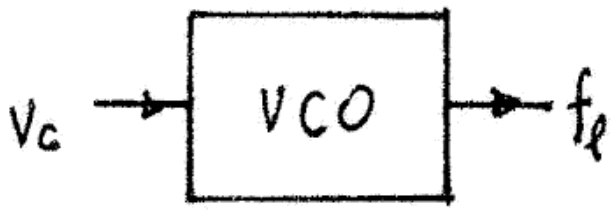
\includegraphics[width=0.4\linewidth]{_fig/pll_vco_volt-freq_bloque.png}
		\label{fig:pll_vco_volt-freq_bloque}
	}
	\subfloat[Característica]
	{
		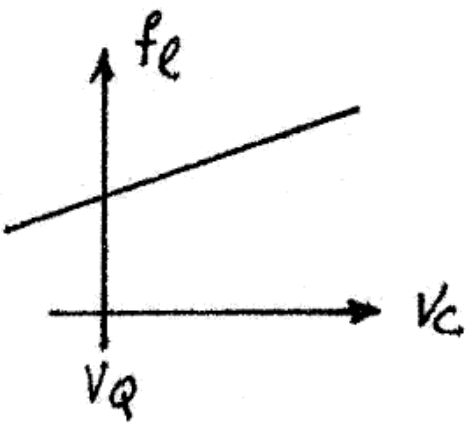
\includegraphics[width=0.4\linewidth]{_fig/pll_vco_volt-freq_caracteristica.png}
		\label{fig:pll_vco_volt-freq_caracteristica}
	}
	\caption{Convertidor de voltaje a frecuencia}
	\label{fig:pll_vco_volt-freq}
\end{figure}

Un esquema de ésto se representa en la Figura \ref{fig:pll_vco_volt-freq_discreto-esquema}: se genera una señal periodica, cuya frecuencia de alguna forma depende del nivel de la señal $V_c$, $\omega = f(V_c)$. En la Figura \ref{fig:pll_vco_volt-freq_discreto-0v}, $V_c$ tiene un nivel de reposo, $V_q$, y se observa una cierta frecuencia de salida. En la Figura \ref{fig:pll_vco_volt-freq_discreto-p1v}, se aplica "$V_c > V_q$". Si la relación salida/entrada es positiva entonces la frecuencia de salida ha aumentado, mientras que en la Figura \ref{fig:pll_vco_volt-freq_discreto-m1v}, al aplicar un control con "$V_c < V_q$", la frecuencia de salida ha disminuido. Finalmente en la Figura \ref{fig:pll_vco_volt-freq_aplicando-seno}, se somete el VCO a una señal de control constantemente en movimiento (senoidal), de modo que la frecuencia instantánea de salida varía constantemente.

\begin{figure}[h]
	\centering
	\subfloat[Esquema general]
	{
		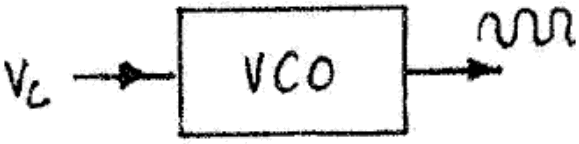
\includegraphics[width=0.22\linewidth]{_fig/pll_vco_volt-freq_discreto-esquema.png}
		\label{fig:pll_vco_volt-freq_discreto-esquema}
	}
	\subfloat[Entrada $0V$]
	{
		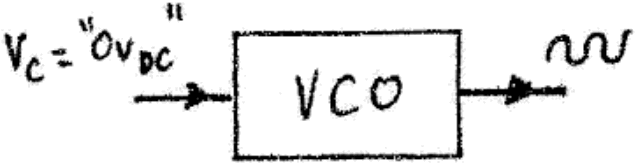
\includegraphics[width=0.22\linewidth]{_fig/pll_vco_volt-freq_discreto-0v.png}
		\label{fig:pll_vco_volt-freq_discreto-0v}
	}
	\subfloat[Entrada $1V$]
	{
		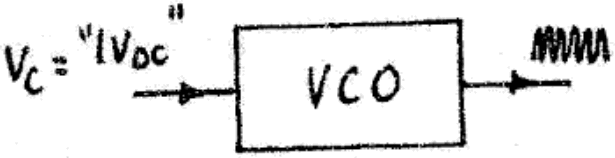
\includegraphics[width=0.22\linewidth]{_fig/pll_vco_volt-freq_discreto-p1v.png}
		\label{fig:pll_vco_volt-freq_discreto-p1v}
	}
	\subfloat[Entrada $-1V$]
	{
		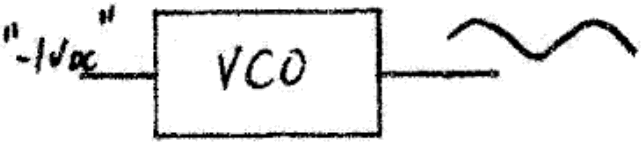
\includegraphics[width=0.22\linewidth]{_fig/pll_vco_volt-freq_discreto-m1v.png}
		\label{fig:pll_vco_volt-freq_discreto-m1v}
	}
	\caption{Convertidor de voltaje a frecuencia, aplicando valor discreto}
	\label{fig:pll_vco_volt-freq_discreto}
\end{figure}

\begin{figure}[h]
	\centering
	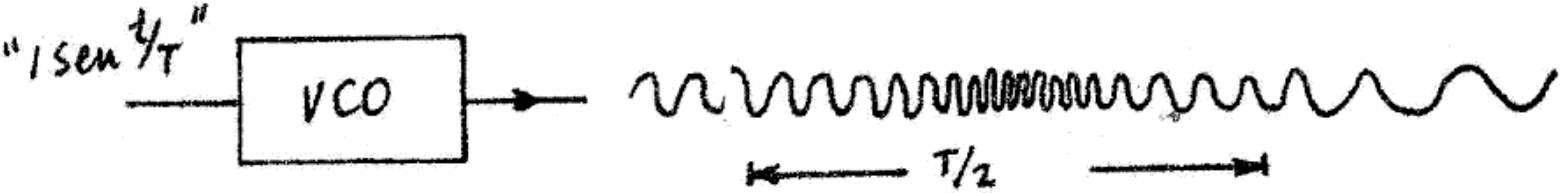
\includegraphics[width=0.8\linewidth]{_fig/pll_vco_volt-freq_aplicando-seno.png}
	\caption{Respuesta de VCO aplicando una senusoidad de entrada en Figura \ref{fig:pll_vco_volt-freq_discreto}}
	\label{fig:pll_vco_volt-freq_aplicando-seno}
\end{figure}

A continuación se indican características deseables de los VCO:

\begin{enumerate}
	\item[a)] Conversión lineal de voltaje a frecuencia
	\item[b)] Buena estabilidad térmica
	\item[c)] Capacidad de trabajar hasta frecuencias elevadas
	\item[d)] Buena ganancia de voltaje a frecuencia
	\item[e)] Capacidad de variar la frecuencia en un rango amplio
	\item[f)] Facilidad de entonación, mínimo número de componentes para fijar la frecuencia de oscilación.
\end{enumerate}

Para llevar a cabo este tipo de oscilador, se podría modificar una de las configuraciones de osciladores presentadas en el capítulo anterior, reemplazando uno de los elementos de valor fijo por un componente o dispositivo cuyo valor fuera función de una tensión aplicada. Por ejemplo, componentes cuyo valor varía con la tensión aplicada incluyen los varactores cuyo valor varía su capacitancia, y los FET que tienen una zona triódica de operación donde trabajan como resistencia lineal variable. En la última sección de este capítulo se describe el 566, un circuito integrado que trabaja como VCO, y que cumple con las características deseables de estos dispositivos.

\section{El comparador de fase} % 226

Genera una salida en función del desfasaje existente entre dos señales. Una de las configuraciones más sencillas, y a la vez aptas para circuitos integrados, es el simple conmutador que se muestra en la Figura \ref{fig:pll_conmutador-detector-fase}.

\begin{figure}[h]
	\centering
	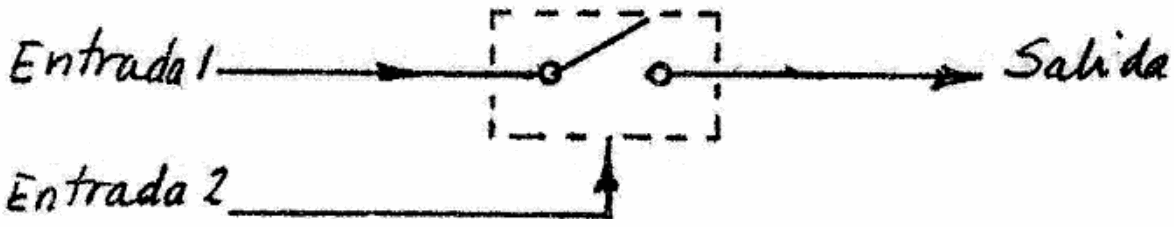
\includegraphics[width=0.8\linewidth]{_fig/pll_conmutador-detector-fase.png}
	\caption{Conmutador como Detector de Fase}
	\label{fig:pll_conmutador-detector-fase}
\end{figure}

La entrada 2 es generalmente una señal digital de modo que cuando la señal es alta el suiche se cierra, y cuando la señal es baja, el switch se abre.

En la Figura \ref{fig:pll_conmutador-detector-fase_eval} se indica la operación de este mecanismo, manteniendo fijo la señal de control (entrada 2), y mostrando las señales resultantes en tres casos desplazando la fase relativa de la señal de entrada (entrada 1) desde $0^\circ$ hasta $180^\circ$ pasando por $90^\circ$. Un filtro paso bajo (integrador) a la salida de este bloque nos proporciona el nivel promedio.

En el caso de desfasaje de $0^\circ$ (caso a), el promedio de la señal de salida es positivo. En el caso de desfasaje de $90^\circ$ (caso b), el voltaje error es 0; esta es una propiedad común de los detectores de fase tipo conmutador. Y en el caso de desfasaje de $180^\circ$ (caso c), el promedio de la señal de salida es negativo.

\begin{figure}[h]
	\centering
	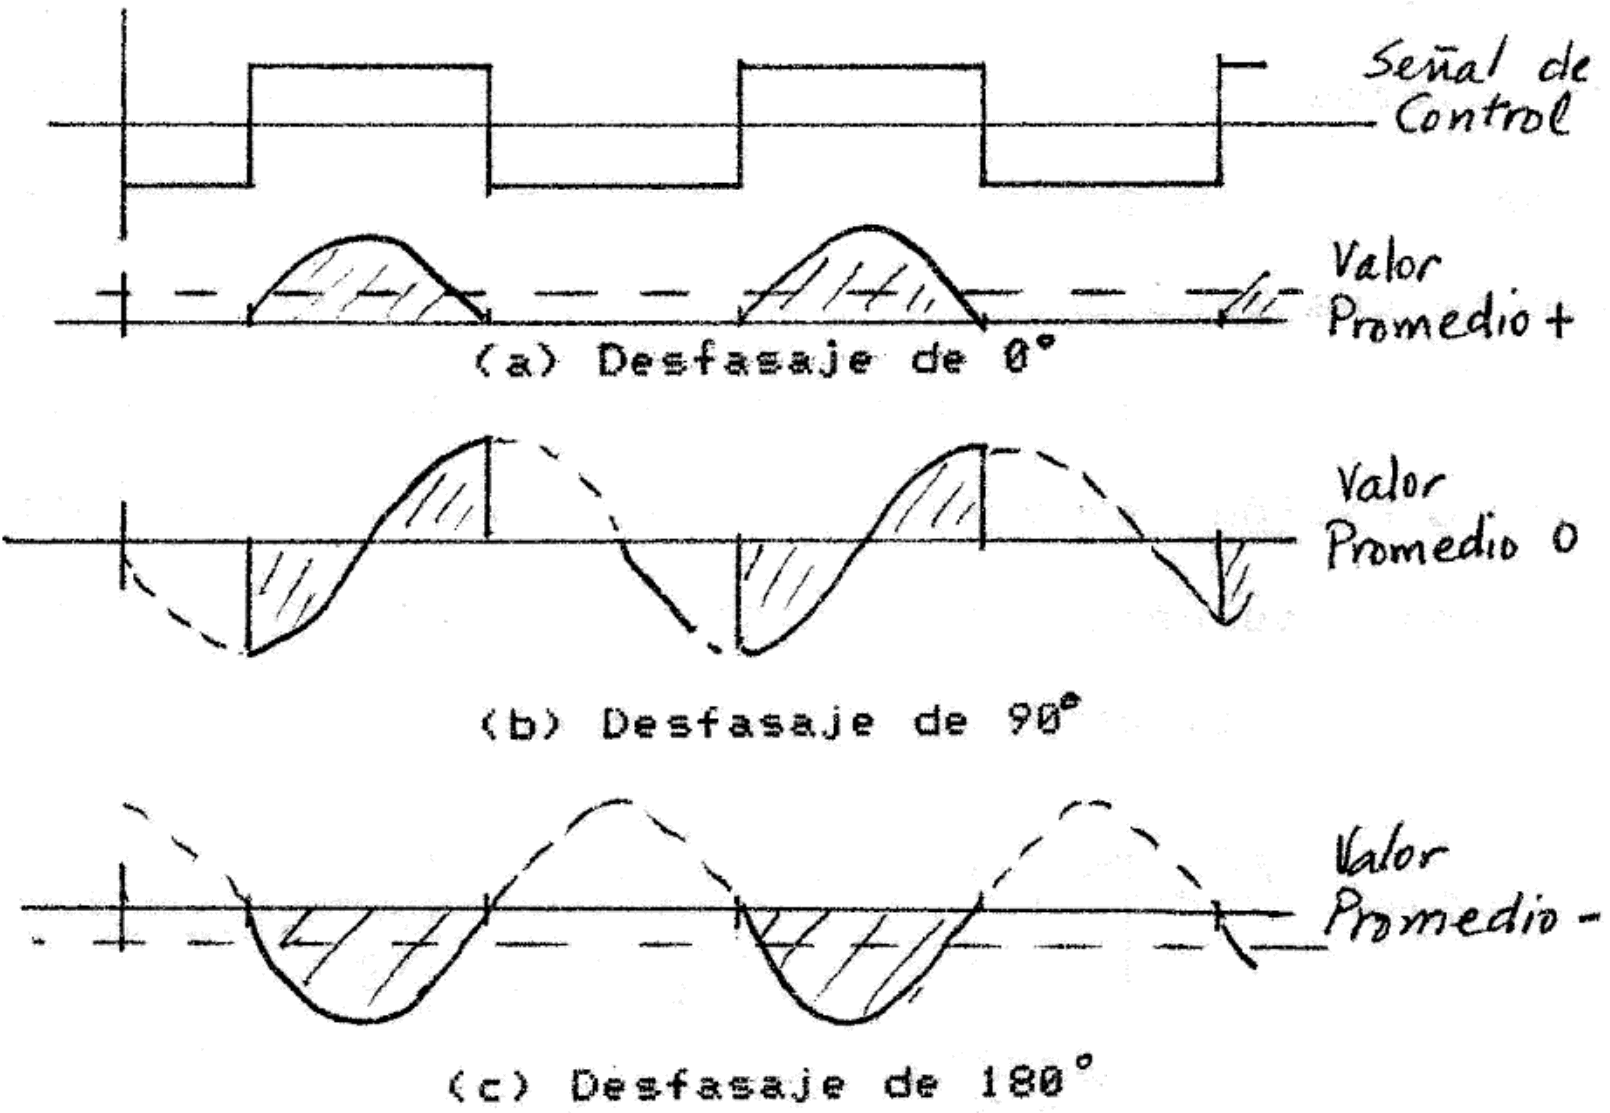
\includegraphics[width=0.8\linewidth]{_fig/pll_conmutador-detector-fase_eval.png}
	\caption{Operación del conmutador como Detector de Fase}
	\label{fig:pll_conmutador-detector-fase_eval}
\end{figure}

Un enfoque distinto de este circuito hace notar que la acción de conmutar el paso de una señal es equivalente a MULTIPLICAR alternativamente por 1 y por 0, es decir, multiplicar por una señal como se indica en la Figura \ref{fig:pll_onda-cuadrada_eval-0-1}.

\begin{figure}[h]
	\centering
	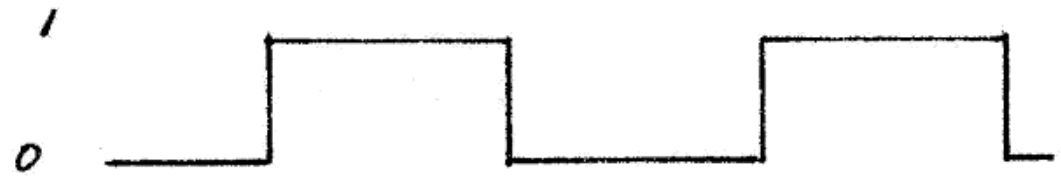
\includegraphics[width=0.8\linewidth]{_fig/pll_onda-cuadrada_eval-0-1.png}
	\caption{Onda cuadrada que varia entre $0$ y $1$}
	\label{fig:pll_onda-cuadrada_eval-0-1}
\end{figure}

Entonces en ocasiones interpretaremos el Detector de Fase como un Multiplicador. Esta señal cuadrada tiene componentes DC, una fundamental y armónicas impares. Al multiplicar la señal de entrada de frecuencia $\omega_i$ con la señal de control de frecuencia $\omega_c$ surgen componentes de frecuencia ($\omega_i$ - $\omega_c$) y ($\omega_i$ + $\omega_c$).

\section{PLL - Lazos de enganche de fase} %p228

Los lazos de enganche de fase son sistemas de retroalimentación negativa en donde la señal de salida es generalmente una tensión, y el parámetro de entrada a comparar es una frecuencia (o fase), tal como se muestra en la Figura \ref{fig:pll_diagrama-de-bloque}. Esta configuración se estudia a nivel teórico para determinar: su estabilidad, su respuesta a cambios bruscos de la entrada, los polos y ceros, régimen transitorio, etc.

\begin{figure}[h]
	\centering
	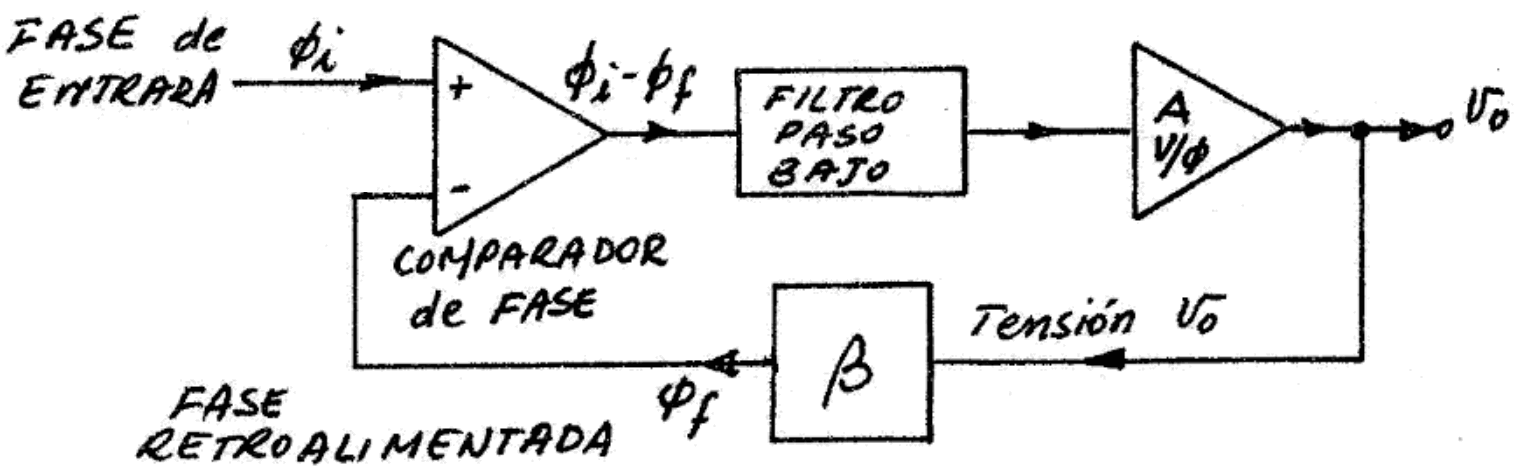
\includegraphics[width=0.8\linewidth]{_fig/pll_diagrama-de-bloque.png}
	\caption{Diagrama de Bloques de un PLL}
	\label{fig:pll_diagrama-de-bloque}
\end{figure}

Sin embargo, a nivel práctico, es mas fructífero darle otro enfoque, que se evidencia en la Figura \ref{fig:pll_esquema-entradas-salidas}. Se habla de la frecuencia de entrada, del voltaje de salida, de una frecuencia local, que puede ser tratada como una salida que a su vez es otra entrada, y de una salida digital, que es opcional.

\begin{figure}[h]
	\centering
	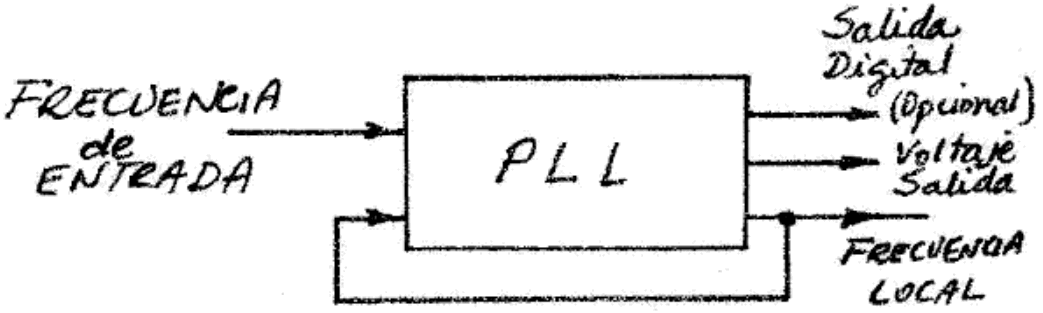
\includegraphics[width=0.8\linewidth]{_fig/pll_esquema-entradas-salidas.png}
	\caption{Esquema de Entrada/Salidas del PLL}
	\label{fig:pll_esquema-entradas-salidas}
\end{figure}

En ausencia de una señal de entrada ($\omega = 0$), el voltaje de salida es su valor de reposo, $V_r$, y la frecuencia local es igual a la \textbf{Frecuencia Libre de Oscilación}, $f_0$ ó $\omega_0$.

Al presentarse una señal a la entrada, surge un régimen transitorio de duración variable según el valor inicial de la fase de entrada, durante el cual varía el voltaje de salida, y varía la frecuencia local de oscilación en una dirección tal que se empareja con la frecuencia de entrada. Al llegar a un régimen estable, la frecuencia local será igual a la frecuencia de entrada, y el voltaje de salida será una constante, proporcional a la diferencia de frecuencia entre la señal de entrada y la frecuencia libre de oscilación. Esta situación se representa en la Figura \ref{fig:pll_regimen-transitorio}.

\begin{figure}[h]
	\centering
	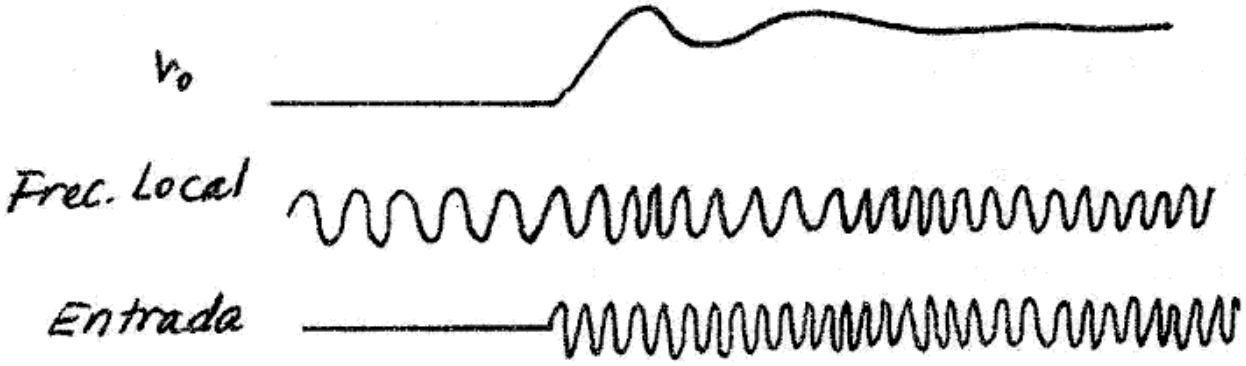
\includegraphics[width=0.8\linewidth]{_fig/pll_regimen-transitorio.png}
	\caption{Regimen Transitorio al Presentarse Señal de Entrada}
	\label{fig:pll_regimen-transitorio}
\end{figure}

Después, con tal de que las variaciones de frecuencia de la señal de entrada no sean demasiado violentas, el oscilador local sigue los cambios de frecuencia de la señal de entrada, como se indica en la Figura \ref{fig:pll_variacion-de-senal}. La salida de voltaje refleja los cambios de frecuencia.

\begin{figure}[h]
	\centering
	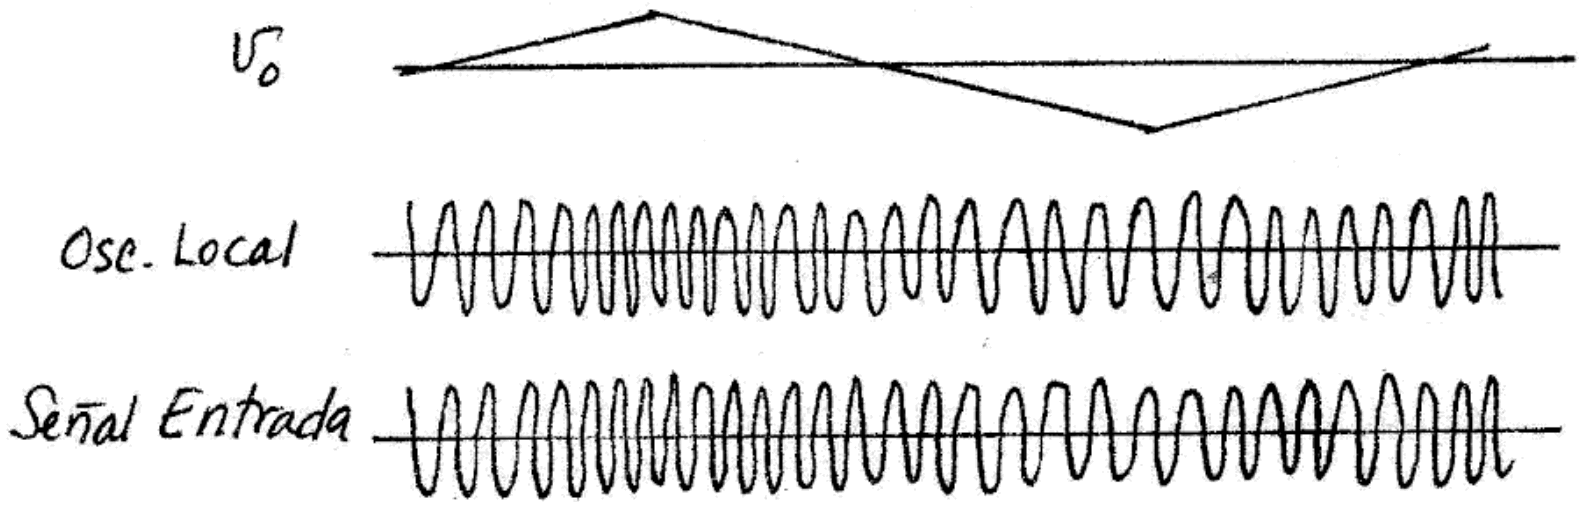
\includegraphics[width=0.8\linewidth]{_fig/pll_variacion-de-senal.png}
	\caption{Variaciones de las señales del PLL al variar la entrada}
	\label{fig:pll_variacion-de-senal}
\end{figure}

Es decir, el oscilador local sigue los cambios de la señal de entrada, y $V_0$ desplaza su nivel en función de los cambios de frecuencia de la señal de entrada. Podríamos pensar que $V_0$ de alguna forma decodifica los cambios de frecuencia de la entrada:

\begin{itemize}
	\item si $V_i \omega = A \sin \omega_o t$, entonces $V_0 = V_Q$
	\item si $V_i \omega = A \sin \omega_i t$, entonces $V_0 = K_1 + V_Q$ $\leftarrow$ $\alpha(\omega_i - \omega_0)$
	\item si $V_i \omega = A \sin \left( \omega_b t \right)$, entonces $v_0 = K_2 \sin \omega_b t + V_q$
\end{itemize}

en este último caso, la frecuencia de oscilación de $V_0$ cambia en forma senusoidal \textit{-una señal modulación de frecuencia-}, y por lo tanto $V_0$ cambia en forma senusoidal.

Este comportamiento del PLL se explica en base al Diagrama de Bloques que aparece en la Figura \ref{fig:pll_diagrama-de-bloque-amplio}.

\begin{figure}[h]
	\centering
	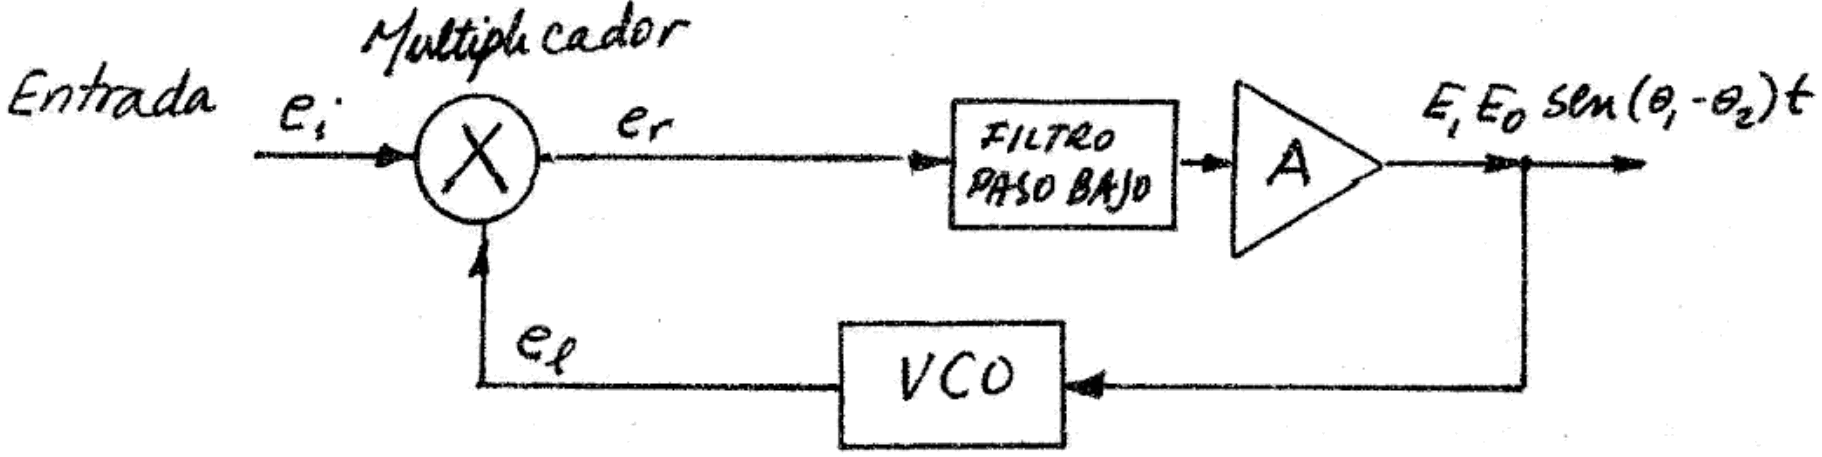
\includegraphics[width=0.8\linewidth]{_fig/pll_diagrama-de-bloque2.png}
	\caption{Diagrama de Bloques del PLL}
	\label{fig:pll_diagrama-de-bloque-amplio}
\end{figure}

Considere que a la entrada tenemos una señal que se describe de la siguiente manera:

\[
e_i = \sqrt{2} E_i \sin(\omega_o t + \theta_1(t))
\]

y que la salida del VCO se describe de la siguiente forma

\[
e_f = \sqrt{2} E_o \sin(\omega_o t + \theta_2(t))
\]

Entonces la salida del multiplicador será igual a

\[
e_r = 2 E_i E_o \sin(\omega_o t + \theta_1(t)) \cos(\omega_o t + \theta_2(t))
\]

\[
e_r = E_i E_o [\sin(\theta_1 - \theta_2)t + \sin(2\omega_o t + \theta_1 + \theta_2)t]
\]

El multiplicador genera el producto de la señal de entrada y de la frecuencia local de oscilación. Sale una componente suma y una componente resta. El filtro paso bajo deja pasar solo la componente de baja frecuencia. La salida del filtro es amplificada y aplicada al VCO de modo que el VCO tiende a cambiar su frecuencia en la dirección de la frecuencia de entrada. Si la frecuencia de entrada es suficientemente cerca a $f_o$, la naturaleza retroalimentativa del PLL provoca el ``enganche'' del VCO con la señal de entrada. Una vez enganchado, la salida del VCO es idéntica a la señal de entrada, excepto por una diferencia de fase, que hace falta para generar la tensión de control que desplaza el VCO de su frecuencia libre de oscilación y mantiene el PLL enganchado.

El PLL tiene limitaciones en su capacidad para seguir las variaciones de la frecuencia de entrada. Este límite se conoce como el \textbf{Rango de Enganche}, $f_l$, y define un rango de frecuencias por arriba y por debajo de la frecuencia libre de oscilación. El rango es generalmente simétrico en relación a la frecuencia libre de oscilación. Esta relación se indica en la Figura \ref{fig:pll_rango-de-enganche}.

\begin{figure}[h]
	\centering
	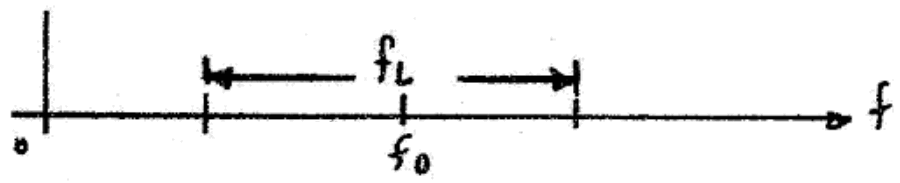
\includegraphics[width=0.8\linewidth]{_fig/pll_rango-de-enganche.png}
	\caption{Rango de Enganche}
	\label{fig:pll_rango-de-enganche}
\end{figure}

Si se presenta a la entrada una señal fuera del rango de enganche, entonces el PLL pierde el seguimiento de la frecuencia de entrada y vuelve a su frecuencia libre de oscilación, y la señal de salida $v_o$ vuelve a su valor de reposo, tal y como si la señal de entrada fuese cero.

Estando el PLL desenganchado, existe una limitación más fuerte en cuanto a las frecuencias a las cuales puede engancharse nuevamente. Esto definirá el \textbf{Rango de Captura}, $f_c$, y representa por lo tanto un rango más reducido alrededor de la frecuencia libre de oscilación, tal como se indica en la Figura \ref{fig:pll_rango-captura-enganche}.

\begin{figure}[h]
	\centering
	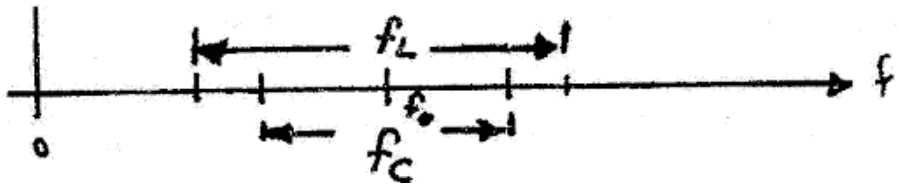
\includegraphics[width=0.8\linewidth]{_fig/pll_rango-captura-enganche.png}
	\caption{Rango de Captura y de Enganche}
	\label{fig:pll_rango-captura-enganche}
\end{figure}

El rango de captura está íntimamente asociado a la característica del filtro paso bajo del PLL. Imagínese que estando desenganchado, a la entrada del PLL se presenta bruscamente una señal de frecuencia $w_x$. Como el PLL estará oscilando a su frecuencia libre de oscilación, $w_o$, las componentes a la salida del Detector de Fase serán $(w_o + w_x)$, que siempre será filtrado por el Filtro Paso Bajo, y $(w_o - w_x)$. Solo si la diferencia $(w_o - w_x)$ está dentro de la banda de paso del filtro es que saldrá una señal capaz de mover el VCO de su posición de reposo en el sentido de la frecuencia de entrada, y de esta forma arrancar con el proceso de enganche que llevará al oscilador local del PLL a terminar emparejándose con la frecuencia de entrada.

Algunos modelos de PLL tienen una salida digital que indica si el PLL está enganchado o no.

\section{Aplicaciones de PLL} % 233

\subsection{Demodulación FM} % 233

En FM, la señal transmitida tiene variaciones de frecuencia en función de la señal mensaje. En la Figura \ref{fig:pll_app-demodulacion-fm}, se representa el esquema para la demodulación de esta señal, donde se aprecia que la salida del PLL es exactamente la señal FM demodulada. Los sistemas que transmiten mensajes por la red eléctrica de 120 VAC emplean modulación FM.

\begin{figure}[h]
	\centering
	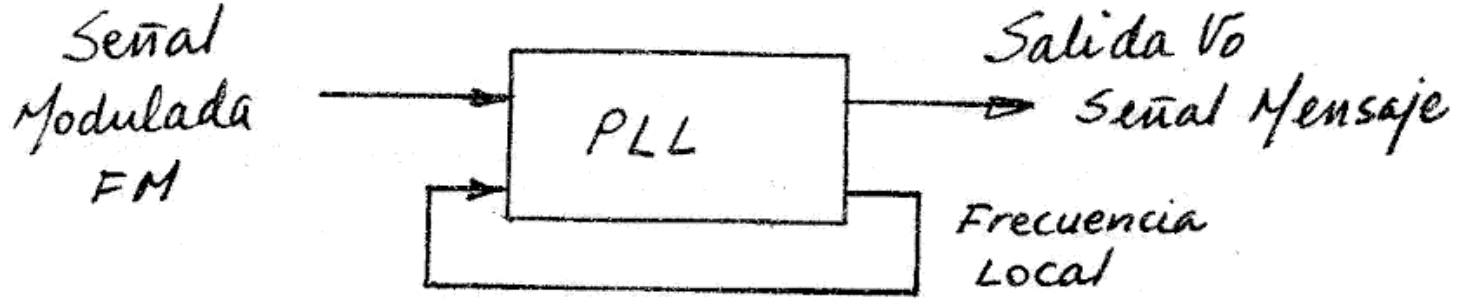
\includegraphics[width=0.8\linewidth]{_fig/pll_app-demodulacion-fm.png}
	\caption{Demodulación FM}
	\label{fig:pll_app-demodulacion-fm}
\end{figure}

\subsection{Detector de Tonos y Controles Remotos - Filtro Pasa Banda Selectivo} % 233

Trabajando con un PLL con salida digital y con un rango de captura muy reducido, se puede ser muy selectivo y responder solo a señales transmitidas. En la Figura \ref{fig:pll_app-control-remoto}, al cerrar el conmutador en el transmisor, se envía una onda de cierta frecuencia, que al captarse por el PLL del receptor hace accionar un relé.

\begin{figure}[h]
	\centering
	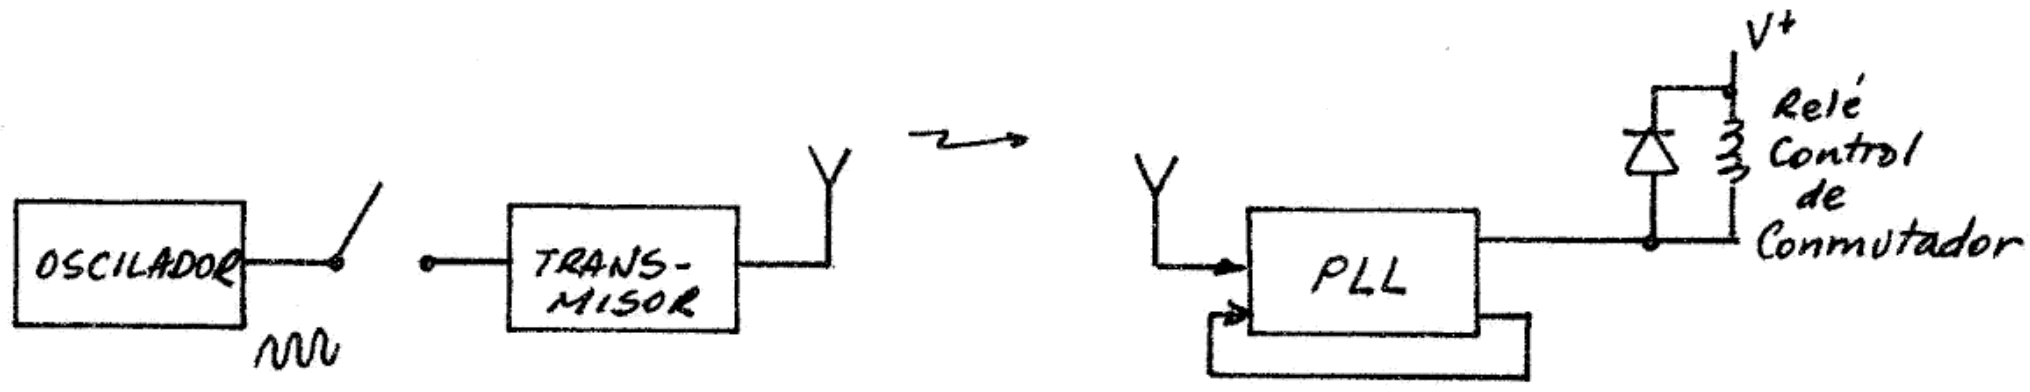
\includegraphics[width=0.8\linewidth]{_fig/pll_app-control-remoto.png}
	\caption{Sistema de Control Remoto}
	\label{fig:pll_app-control-remoto}
\end{figure}

\subsection{Multiplicador de Frecuencia} % 234

El PLL puede ser usado para generar una señal cuya frecuencia es un múltiplo de la frecuencia de entrada. La configuración se muestra en la Figura \ref{fig:pll_app-multiplicador-frecuencia}. Se hace notar que se ha cambiado la conexión normal entre la salida del VCO y una entrada al Detector de Fase. En lugar de una conexión directa se ha intercalado un Divisor de Frecuencia. De esta forma, la frecuencia de salida del VCO es dividida por $N$, y se empareja esta frecuencia dividida con la frecuencia de la señal de entrada, $f_0/N = f_i$, y entonces la salida directa del VCO resulta ser $N$ veces la frecuencia de entrada, $f_0 = Nf_i$.

\begin{figure}[h]
	\centering
	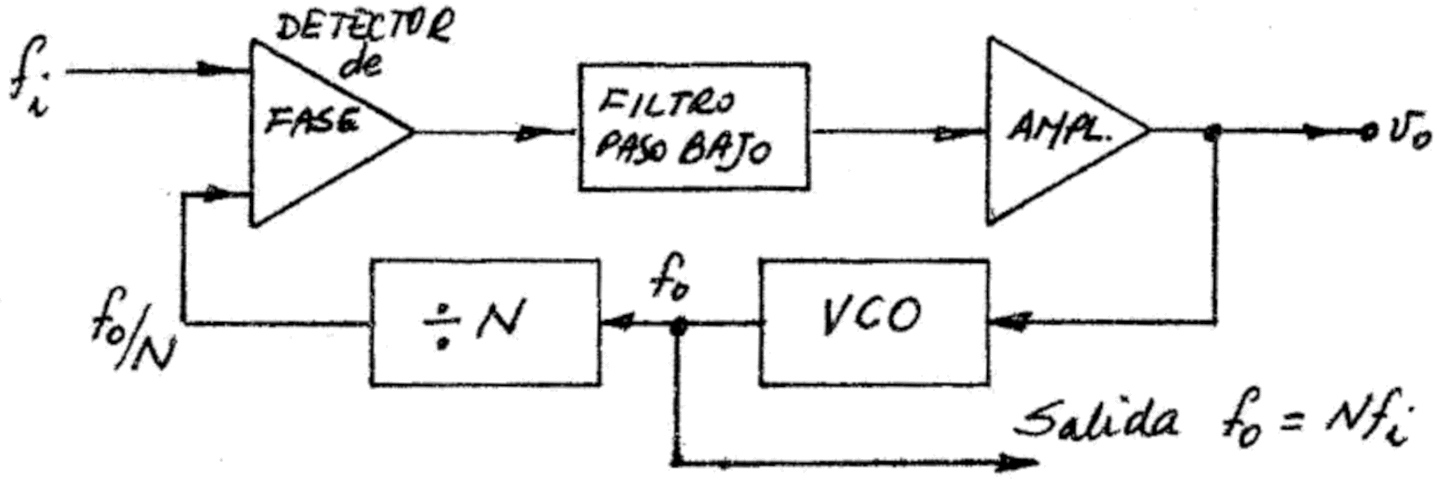
\includegraphics[width=0.8\linewidth]{_fig/pll_app-multiplicador-frecuencia.png}
	\caption{Multiplicador de Frecuencia}
	\label{fig:pll_app-multiplicador-frecuencia}
\end{figure}

\subsection{Extractor de Frecuencia Reloj o Fundamental} % 235

En varios sistemas de transmisión la señal enviada tiene múltiples informaciones; el PLL es muy útil para distinguir entre las señales, particularmente para extraer un reloj o portadora.

\subsubsection{Demodulación AM Síncrona}

Por medio del esquema que aparece en la Figura \ref{fig:pll_app-extractor-frecuencia} se detecta la portadora de una señal AM; con esta portadora se multiplica la señal de entrada, trasladando su espectro a bajas frecuencias, que al filtrarlo nos produce la señal mensaje. El Desfasador de $90^\circ$ es para compensar el desfase de $90^\circ$ en el PLL entre la señal de entrada y la salida del VCO.

\begin{figure}[h]
	\centering
	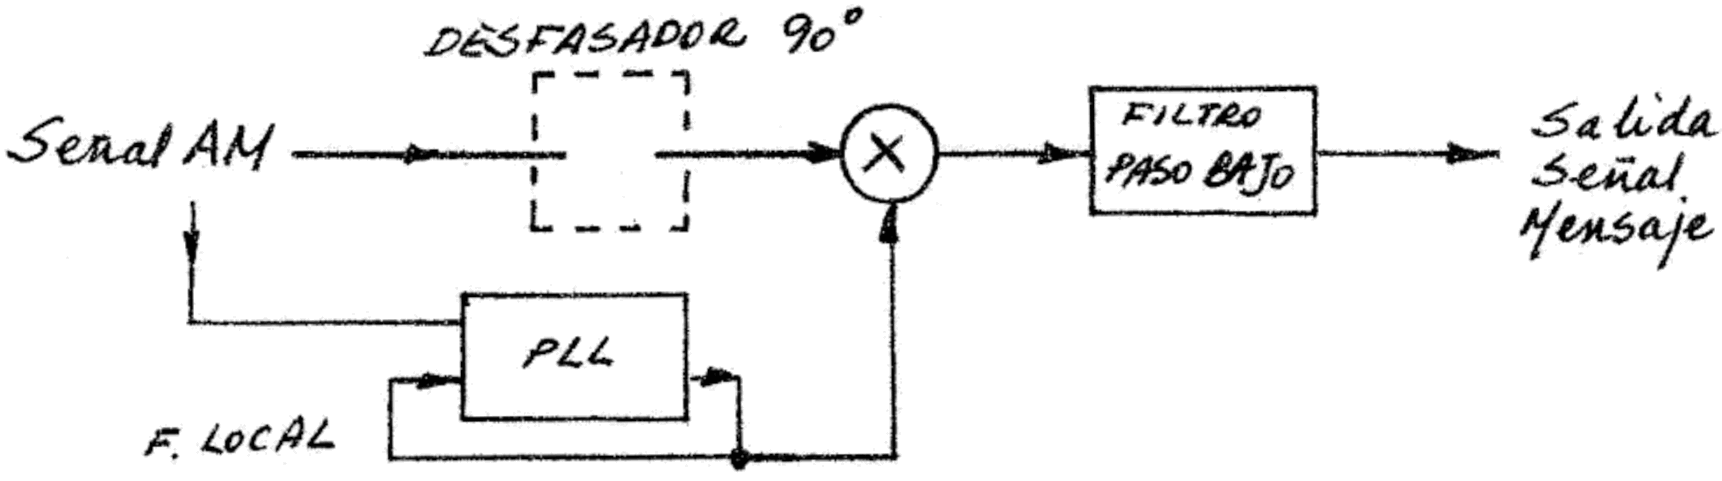
\includegraphics[width=0.8\linewidth]{_fig/pll_app-demodulador-sincrono-am.png}
	\caption{Demodulador Síncrono AM}
	\label{fig:pll_app-extractor-frecuencia}
\end{figure}

\section{Circuitos integrados: VCO, PLL y sus Ecuaciones de Diseño} %p235

\subsection{El 565} %p235

El 565 es un PLL de propósito general que es capaz de trabajar en el rango de 0.001 Hz a 500 kHz. Las conexiones del circuito y los componentes externos requeridos se muestran en la Figura \ref{fig:pll_565-diagrama}. La resistencia $R$ y el condensador $C_1$ fijan la frecuencia libre de oscilación. El condensador externo $C_2$ y la resistencia de salida de la pata 7 de 3.6 k$\Omega$ fijan la frecuencia de corte del filtro paso bajo y de esta forma establecen los límites del rango de captura. El condensador de 1~nF entre las patas 7 y 8 se requiere para estabilizar el circuito, es decir, evitar oscilaciones no deseadas. A continuación, ecuaciones de diseño:

\begin{figure}[h]
	\centering
	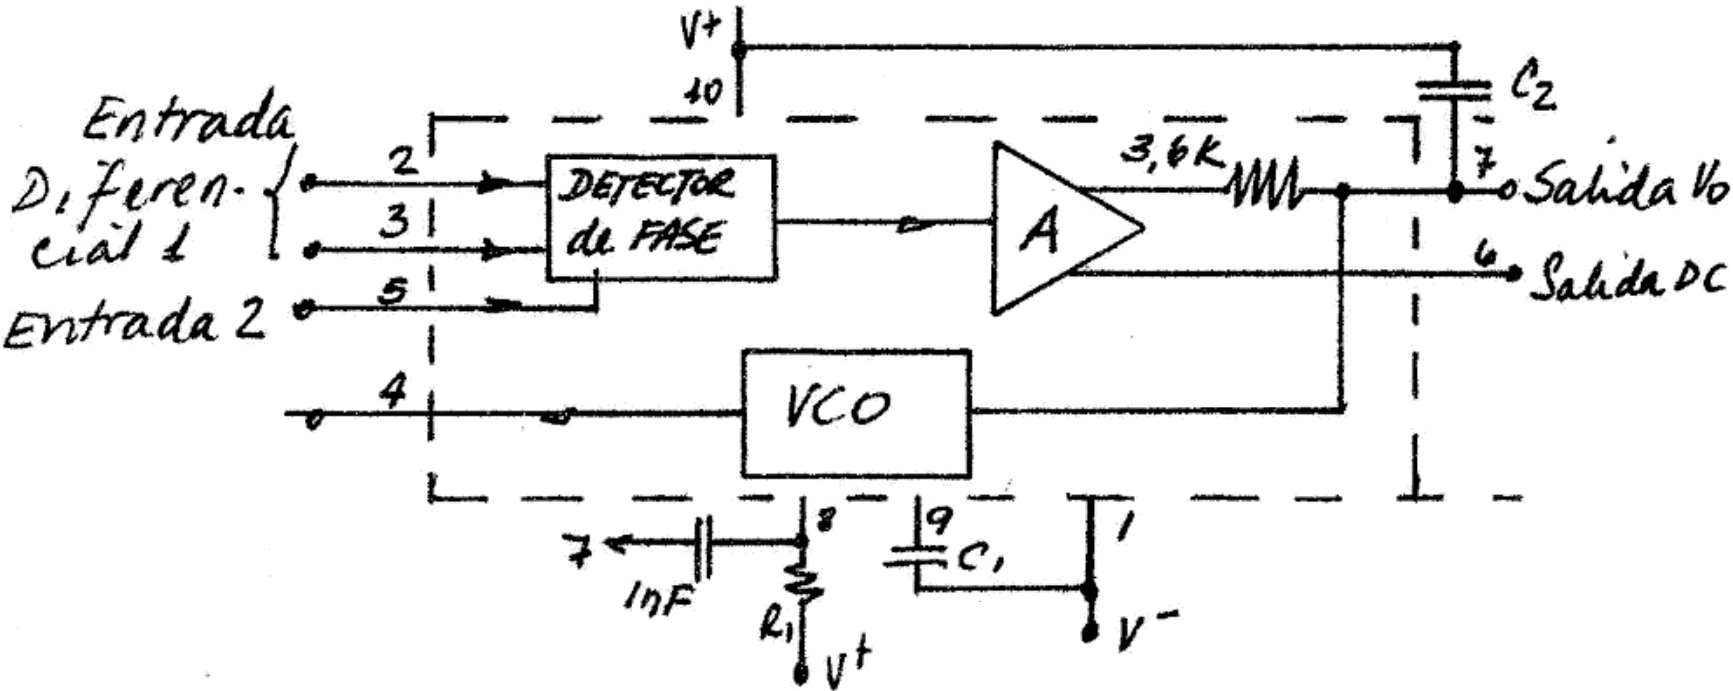
\includegraphics[width=0.8\linewidth]{_fig/pll_565-diagrama.png}
	\caption{El PLL 565}
	\label{fig:pll_565-diagrama}
\end{figure}

Valor típico de alimentación: $V^+ = +6$V; \quad $V^- = -6$V

Y en la Figura \ref{fig:pll_565-conexion-tipica} una conexión típica. Las entradas 2 y 3 tienen que estar aproximadamente al mismo nivel de continua; esto se logra con las resistencias respectivas a tierra. Después se acopla la señal al circuito por medio de un condensador.

\begin{figure}[h]
	\centering
	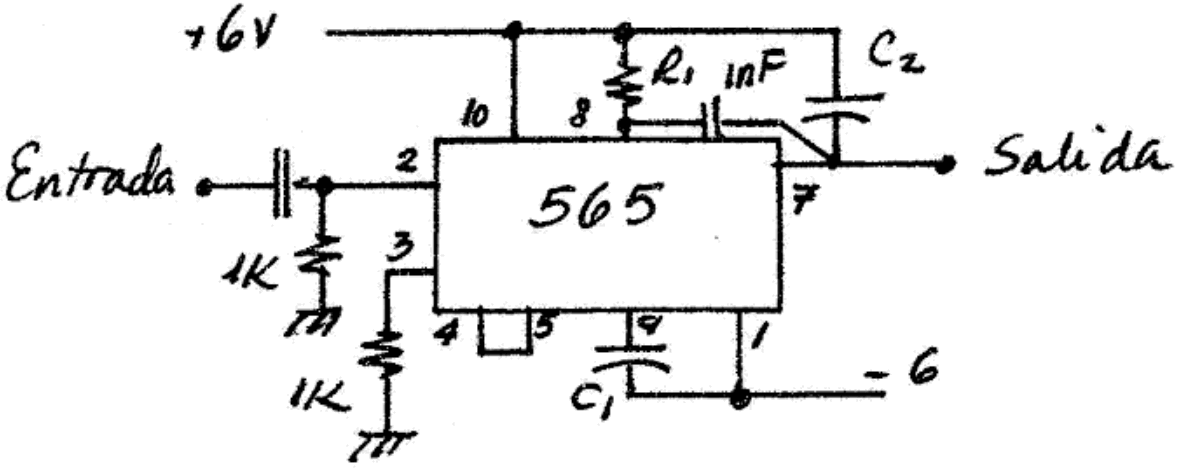
\includegraphics[width=0.8\linewidth]{_fig/pll_565-conexion-tipica.png}
	\caption{Conexión típica del 565}
	\label{fig:pll_565-conexion-tipica}
\end{figure}

\subsection{El 567} %p237

El 567 es un PLL con Salida Digital. Las conexiones del circuito y los componentes externos requeridos se muestran en la Figura \ref{fig:pll_567-diagrama}. La resistencia $R_1$ y el condensador $C_1$ establecen la frecuencia libre de oscilación. El condensador $C_2$ establece la frecuencia de corte del filtro paso bajo y por lo tanto los límites del rango de captura, en este caso conocido como el ancho de banda. El condensador $C_3$ es un filtro paso bajo previo a la salida digital.

Cuando una señal de entrada es de una frecuencia dentro del ancho de banda, la salida digital (la pata 8) pasa a un nivel bajo. El rango de enganche no se precisa por considerar que el circuito va a trabajar como detector de tonos, con cambios bruscos de frecuencia fuera y dentro del rango de captura. A continuación las ecuaciones correspondientes de diseño.

\begin{figure}[h]
	\centering
	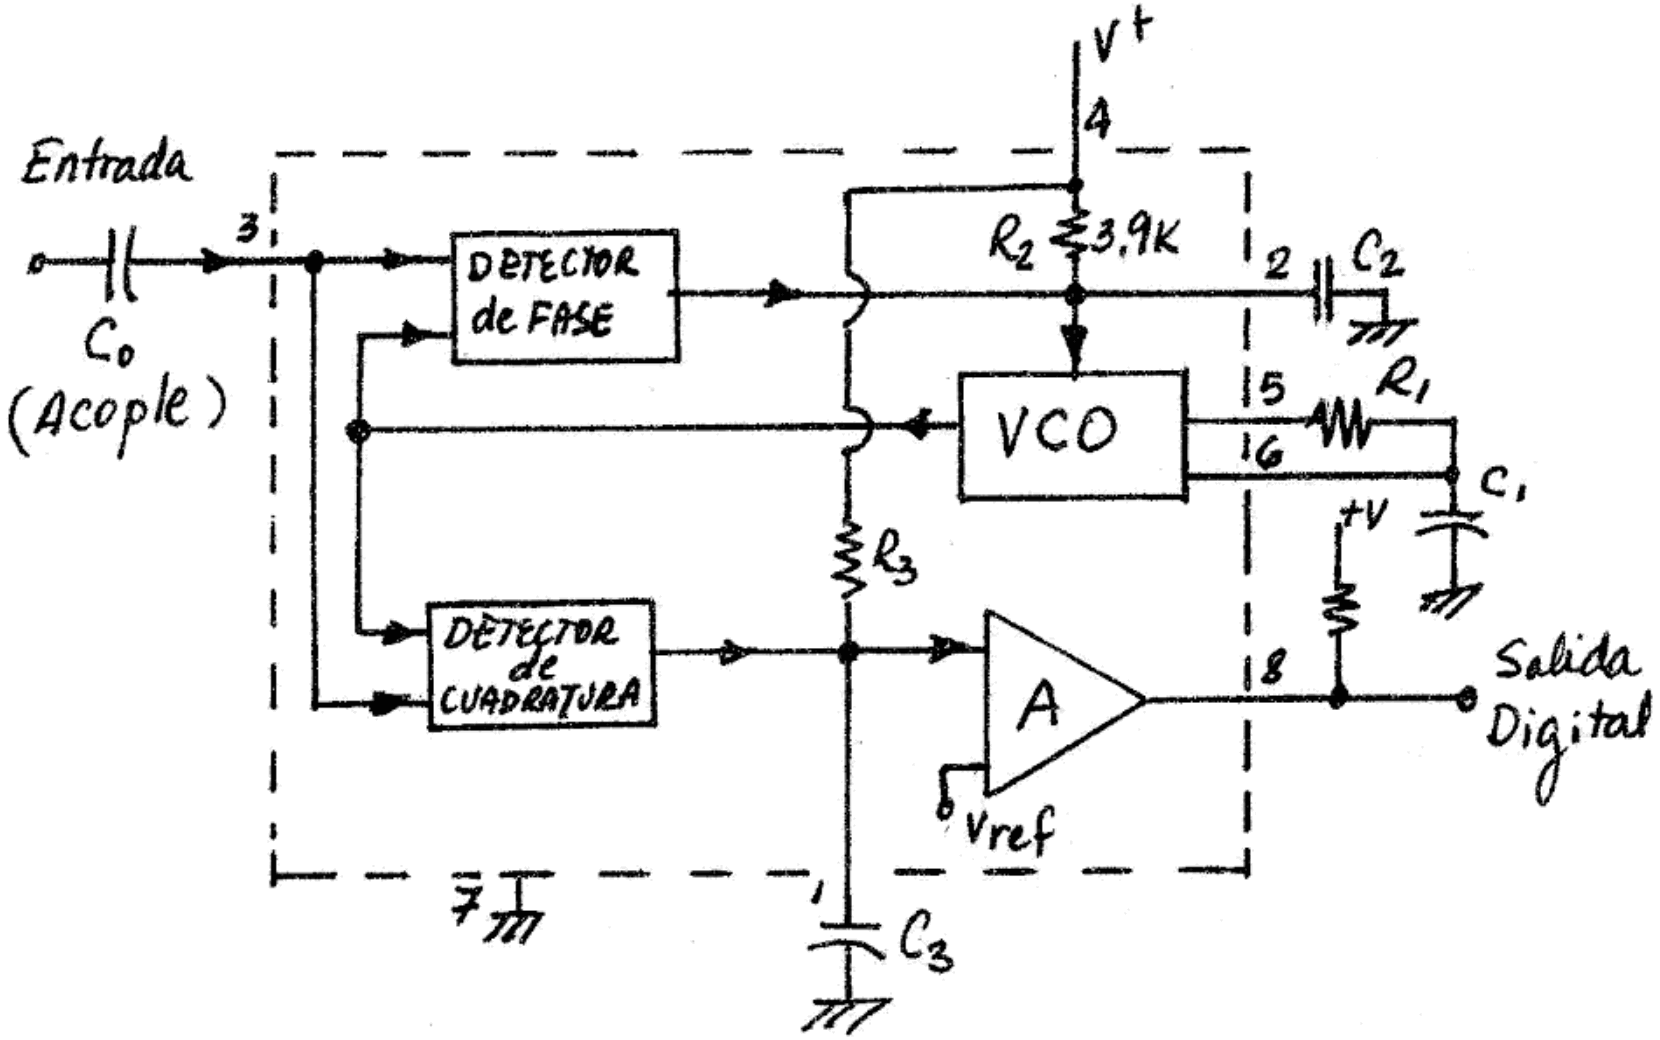
\includegraphics[width=0.8\linewidth]{_fig/pll_567-diagrama.png}
	\caption{El 567}
	\label{fig:pll_567-diagrama}
\end{figure}

Freq. libre de oscilación: \( f_0 = \frac{1.1}{R_1 C_1} \)

Ancho de Banda de captura: \( BW = \frac{1070 \sqrt{V_i / f_0}}{C_2} \)

donde $BW$ se expresa en $\%$ de $f_0$, $V_i$ es un valor $\leq 200 \text{mVrms}$, y $C_2$ tiene unidades de $\mu F$.

Finalmente: \( C_3 \approx 2 C_2 \)

\subsubsection{Ejemplo}

Determine $R_1$, $C_1$, $C_2$ y $C_3$ para $f_0 = 100$ kHz con $BW = 1\%$.

\textbf{Solución:} deje que $R_1 = 3.9k \Omega$, entonces: \( C_1 = \frac{1.1}{3.9k \times 100k} = 2.8 nF \). Suponer $V_i = 200 \text{mVrms} = 0.2$, entonces:

\( C_1 = 1070 \sqrt{\frac{0.2}{10^5} C_2} \) de donde  \( C_2 = 2.3 \mu F \)

y \( C_3 = 2 C_2 \approx 4.5 \mu F \)


\subsection{El 566} %p238

El 566 es un VCO. Tiene una tensión de control, y tiene dos salidas periódicas de la misma frecuencia: una cuadrada y una triangular. En la Figura \ref{fig:pll_566-conexion-tipica} se muestra una conexión típica.

\begin{figure}[h]
	\centering
	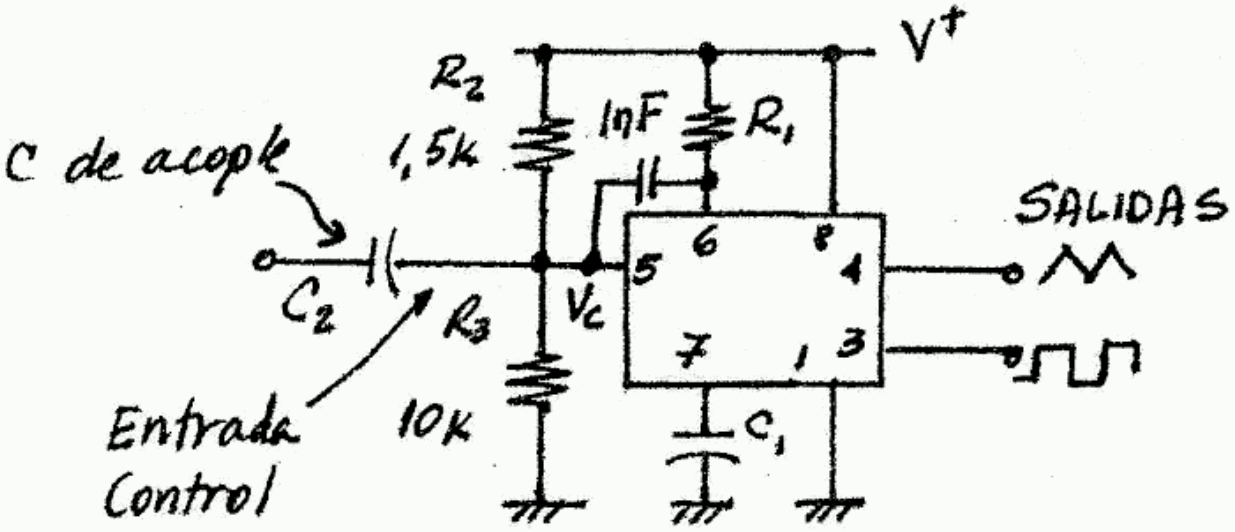
\includegraphics[width=0.8\linewidth]{_fig/pll_566-conexion-tipica.png}
	\caption{El 566}
	\label{fig:pll_566-conexion-tipica}
\end{figure}

La resistencia $R_1$ y el $C_1$ fijan el rango de frecuencias de trabajo. La tensión de entrada (la pata 5) tiene que ubicarse entre los niveles de $V^+$ y $3/4$ de $V^+$, donde $V^+$ representa la diferencia entre la fuente positiva (la pata 8) y la fuente negativa (la pata 1), que normalmente está unida a tierra.

Con los valores indicados de $R_2 = 1.5$k y $R_3 = 10$k, el voltaje de control está prácticamente en el medio de su rango permitido. El condensador de $1 nF$ entre las patas 5 y 6 sirve para estabilizar el dispositivo. Dado valores para el voltaje de control, $V_C$, y los componentes $R_1$ y $C_1$, la frecuencia de salida viene dada por:

\[
f_o \approx \frac{2 (V^+ - V_C)}{R_1 C_1 V^+}
\]

\subsection{4046B} %p239

El chip CMOS 4046B es probablemente uno de los más versátiles y menos utilizados de todos los IC en la gama CMOS. Este dispositivo se enorgullece (o sufre) del título descriptivo de "bucle de enganche en fase de micropotencia" y existe una idea errónea generalizada en la que el dispositivo solo puede usarse en aplicaciones tipo PLL, su uso puede ser más extensivo.

\subsubsection{4046B, estructura interna}

El 4046B contiene un par de comparadores de fase, un diodo zener y un VCO o oscilador controlado por voltaje (ver Figura \ref{fig:pll_mc14046b_bd}) y su pinout ver Figura \ref{fig:pll_mc14046b_pinout}. Todas estas secciones son accesibles de forma independiente mediante las salidas del IC. La sección VCO del dispositivo es probablemente el oscilador controlado por voltaje más versátil y rentable del mercado. Produce una salida simétrica de forma de onda bien definida, con un barrido de frecuencia de más de $1 MHz$, y puede ser escaneado en frecuencia dentro de un rango de $1000000:1$ (de $1 Hz$ a $1 MHz$) usando una única resistencia de temporización o en cualquier proporción entre $1:1$ e infinito ($0 Hz$ a $1 MHz$) cuando se usa un par de resistencias de temporización.


\begin{figure}[h]
	\centering
	\subfloat[Diagrama de Bloque]
	{
		\includegraphics[width=0.7\linewidth]{_fig/pll_mc14046b_bd.pdf}
		\label{fig:pll_mc14046b_bd}
	}
	\subfloat[Pinout]
	{
		\includegraphics[width=0.26\linewidth]{_fig/pll_mc14046b_pinout.pdf}
		\label{fig:pll_mc14046b_pinout}
	}
	\caption{4046B}
	\label{fig:pll_mc14046b}
\end{figure}


Si esto no fuera suficiente, el VCO también puede activarse y desactivarse de manera independiente mediante una terminal INHIBIT, puede operar desde cualquier suministro de voltaje en el rango de $3$ a $18 V$, y cuando se usa junto con uno de los comparadores de fase del 4046B, puede generar una salida en cuadratura. La linealidad del VCO es típicamente del orden del $1\%$.



El 4046B es un PLL de la familia lógica CMOS. En la Figura \ref{fig:pll_4046b-conexion-tipica} se muestra una conexión típica. La resistencia $R_1$ y el condensador $C_1$ fijan la frecuencia de libre oscilación. La resistencia $R_3$ y el condensador $C_2$ fijan la frecuencia de corte del filtro paso bajo y por ende el rango de captura. La resistencia $R_2$ se usa para desplazar la frecuencia libre de oscilación y reducir el rango de enganche.

\begin{figure}[h]
	\centering
	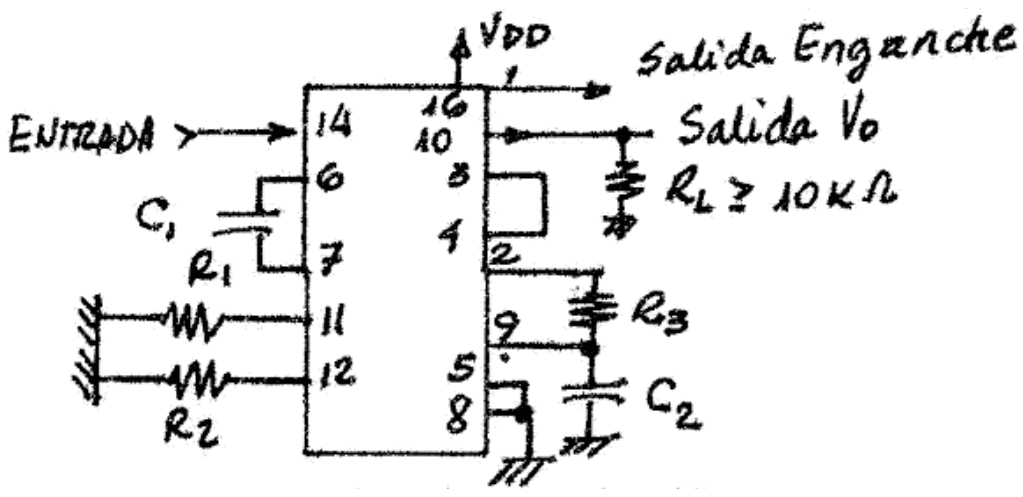
\includegraphics[width=0.8\linewidth]{_fig/pll_4046b-conexion-tipica.png}
	\caption{El 4046}
	\label{fig:pll_4046b-conexion-tipica}
\end{figure}

El dispositivo tiene dos comparadores de fase: uno que establece un desfase de $90^\circ$ y el otro un desfase de $0^\circ$, y que además suministra pulsos de enganche. Ecuaciones de diseño:

Frecuencia libre de oscilación: \( f_o = \frac{1}{R_1 C_1} \)

Rango de captura: \( f_c = \pm \frac{1}{2\pi} \sqrt{\frac{2\pi f_L}{R_3 C_2}} \), $f_L$ depende de $R_2$

\section{Problemario} %p240

- pendiente en apuntes -